\chapter*{Введение} % * не проставляет номер
\addcontentsline{toc}{chapter}{Введение} % вносим в содержание


Задача распознавания структуры химической молекулы является разновидностью задачи компьютерного зрения. До того, как машинное обучение получило широкое распространение, такие задачи чаще всего решали алгоритмическим путём. Так, большинство решений, упомянутых в \cite{rajan2020review}, состояло из этапов предобработки (сглаживание, бинаризация), поиска связей как отрезков прямых и распознавания меток атомов OCR-методами. Решение, основанное на таком подходе, оказывается уязвимым к дефектам изображения, таким как шум, получаемый при сканировании, дефекты печати, следы эксплуатации журналов и книг (мятые или надорванные страницы). Кроме того, при создании алгоритмического решения оказывается гораздо сложнее поддерживать такие параметры, как положения букв на метках атомов, шрифты, расстояние между линиями на двойных и тройных связях,
поскольку OCR-методы зачастую параметризуются различного рода порогами погрешностей.

\begin{figure}[h!] 
	\center
	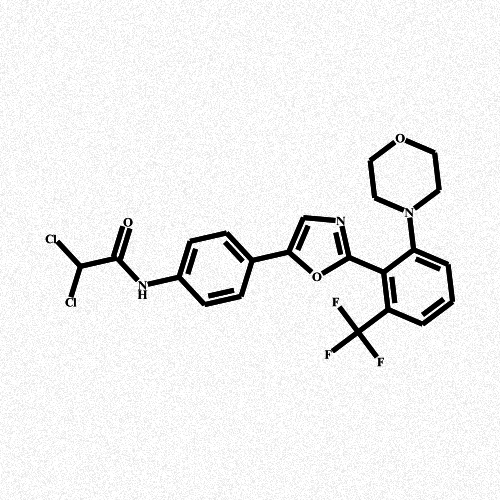
\includegraphics [scale=0.45] {my_folder/images/nh_vert}
	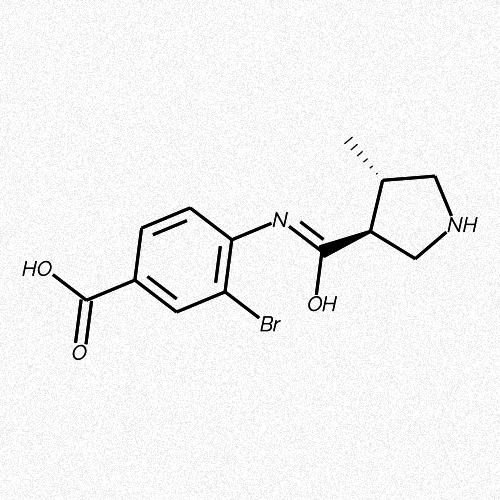
\includegraphics [scale=0.45] {my_folder/images/nh_hor}
	\caption{Изображения молекул, на которых метка атома азота с присоединённым атомом водорода изображена: (1) вертикально, (2) горизонтально} 
	\label{fig:nh}  
\end{figure}

\begin{figure}[h!] 
	\center
	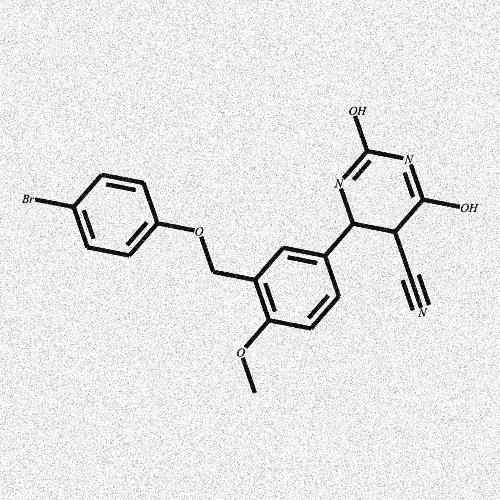
\includegraphics [scale=0.45] {my_folder/images/23bonds}
	\caption{Молекула с двойными и тройными связями. Двойная связь обозначается двумя параллельными отрезками, тройная -- тремя} 
	\label{fig:23bond} 
\end{figure}

Таким образом, программная поддержка алгоритмических решений является крайне трудоёмким процессом, поскольку при появлении новых, пусть даже слабо отличающихся от предыдущих, стандартов рендеринга изображений, в программу-распознаватель придётся дописывать блоки кода, поддерживающие эти изменения.

В то же время решение, построенное с помощью методов машинного обучения, даже не видя каких-то характерных особенностей изображений при обучении, зачастую сможет провести коррректное распознавание. Если же окажется, что изменение слишком сильное, достаточно добавить некоторое количество изображений с новой особенностью в обучающую выборку и дообучить сеть, что требует весьма небольших затрат ресурсов.

Задача распознавания структуры химической молекулы является частью комплексного решения по распознаванию документа и необходима преимущественно для распознавания научных статей по химии, биологии и медицине. Распознавание документов необходимо для следующих целей:
\begin{itemize}
	\item Хранение <<идеальных>> рендеров: пользователь получает возможность читать документы без дефектов. Изображения молекул и другие векторные по своей природе схемы, отпечатанные на бумаге в растровом виде, сохраняются в векторном формате, что позволяет пользователю масштабировать изображение до необходимых ему пределов.
	
	\item Хранение документов в plain-text формате позволяет осуществлять эффективный поиск информации. В частности, модуль распознавания структуры молекулы позволяет искать научные статьи, содержащие информацию о конкретной молекуле. Данная функциональность помогает фармацевтическим исследователям находить интересующие их свойства конкретных веществ, что значительно ускоряет процесс создания лекарственных средств.
\end{itemize}

В рамках данной работы предполагается, что распознавание структуры химической молекулы может производиться как для сканов печатных документов, так и для электронных документов, не содержащих информацию о структуре молекулы в плоском виде.

Таким образом, \textbf{исследование является актуальным}, поскольку построение решения, которое позволяет распознавать структуру химической молекулы на разнообразных данных, поможет создать высококачественный распознаватель документов химической тематики, что в свою очередь значительно улучшит качество и производительность работы исследователей в сфере химии, биологии и фармацевтики.

\textbf{Целью проводимого исследования} является создание описанного ранее решения, замеры его качества, оценка производительности. Также в рамках исследования будет оценена скорость обучения выбранных моделей и \textit{масштабируемость} решения, то есть трудозатраты, требуемые для поддержки дополнительных элементов молекул, таких как RS-стереометки атомов и обозначения смесей различных геометрических изомеров.

\begin{figure}[h!] 
	\center
	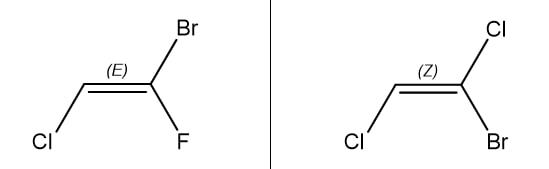
\includegraphics [scale=0.74] {my_folder/images/ez}
	\caption{Изображение молекул с \textit{(E)}, \textit{(Z)} метками \cite{stereochem}}
	\label{fig:ez}  
\end{figure}

\begin{figure}[h!] 
	\center
	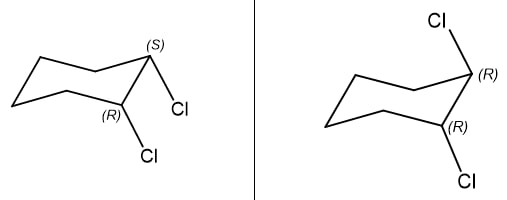
\includegraphics [scale=0.68] {my_folder/images/rs}
	\caption{Изображение молекул с \textit{(R)}, \textit{(S)} метками \cite{stereochem}} 
	\label{fig:rs}  
\end{figure}


% Целью первой главы, как правило, является всесторонний анализ предмета и объекта исследования, второй --- разработка предложений (алгоритмов, технологий и т.п.) по улучшению какого-либо процесса, протекающих с участием предмета и объекта исследования, третьей --- практическая реализация (имплементация) --- предложений (алгоритмов, технологий и т.п.) в виде программного (или иного) продукта, четвертой --- апробация разработанных в работе предложений и выводы целесообразности их дальнейшей разработки (использованию). 


%% Вспомогательные команды - Additional commands
%\newpage % принудительное начало с новой страницы, использовать только в конце раздела
%\clearpage % осуществляется пакетом <<placeins>> в пределах секций
%\newpage\leavevmode\thispagestyle{empty}\newpage % 100 % начало новой строки